\documentclass{beamer}
\usepackage{graphicx}
\usepackage{tikz}
\usetikzlibrary{arrows.meta,positioning}

% -- Blue theme colours --
\definecolor{earlblue}{RGB}{0,63,114}

\setbeamercolor{frametitle}{bg=earlblue,fg=white}
\setbeamercolor{title}{fg=white}
\setbeamercolor{structure}{fg=earlblue}
\setbeamercolor{normal text}{fg=black}
\setbeamercolor{footline}{bg=earlblue,fg=white}
\setbeamertemplate{navigation symbols}{}

% Rounded, themed blocks (used to highlight callout boxes on content slides)
\setbeamertemplate{blocks}[rounded][shadow=false]
\setbeamercolor{block title}{bg=earlblue,fg=white}
\setbeamercolor{block body}{bg=earlblue!8,fg=black}

% Blue footline bar with logo bottom-right, used on content slides
\setbeamertemplate{footline}{%
  \begin{beamercolorbox}[wd=\paperwidth,ht=0.8cm,dp=0.25cm]{footline}
    \hfill
\includegraphics[height=0.55cm]{assets/earlconf.png}\hspace{0.4cm}
  \end{beamercolorbox}%
}

%Information to be included in the title page:
\title{Agentic AI System for Enterprise Cloud Migration}
\newcommand{\presenters}{Timothy Wong \quad $\bullet$ \quad Alessandro Abati}
\institute{London Stock Exchange Group (LSEG)}
\date{7 Oct 2026}

\begin{document}

% -- Cover slide: full blue background, logo centred at bottom --
{
\setbeamertemplate{footline}{}
\usebackgroundtemplate{%
  \begin{tikzpicture}[remember picture,overlay]
    \fill[earlblue] (current page.south west) rectangle (current page.north east);
  \end{tikzpicture}%
}
\begin{frame}[plain]
\centering
\color{white}
\vspace{1.2cm}
{\Huge\bfseries \inserttitle\par}
\vspace{1.2cm}
{\Large \presenters\par}
\vspace{0.8cm}
{\large \insertinstitute\par}
\vspace{0.3cm}
{\large \insertdate\par}
\vspace{0.2cm}
\vfill

\includegraphics[height=1.3cm]{assets/earlconf.png}
\vspace{0.6cm}
\end{frame}
}

% ---- Speaker Introduction ----
\begin{frame}
\frametitle{About the Speakers}
\begin{columns}[T]
\begin{column}{0.5\textwidth}
  \centering
  \IfFileExists{assets/tim.png}{%
    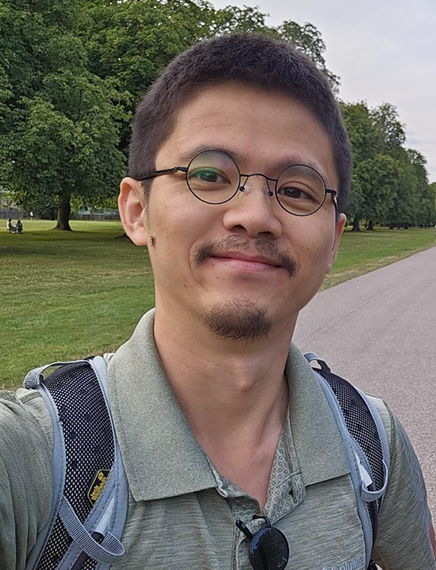
\includegraphics[height=0.6\linewidth]{assets/tim.png}%
  }{%
    \fbox{\parbox[c][0.6\linewidth][c]{0.6\linewidth}{\centering Photo}}%
  }
  \\[0.3cm]
  \textbf{Timothy Wong} \\
  {\footnotesize
  Tim is an AI/ML engineer at LSEG with over ten years experience in enterprise data science applications.
  He hosted talks at EARL 2016, 17, 19 \& 24.}
\end{column}
\begin{column}{0.5\textwidth}
  \centering
  \IfFileExists{assets/alessandro.png}{%
    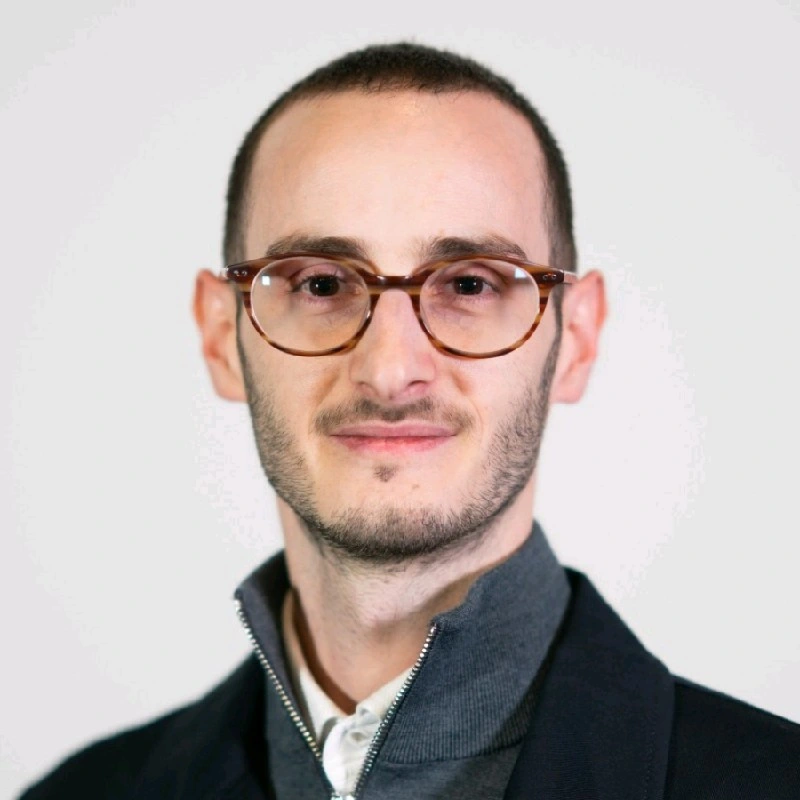
\includegraphics[height=0.6\linewidth]{assets/alessandro.png}%
  }{%
    \fbox{\parbox[c][0.6\linewidth][c]{0.6\linewidth}{\centering Photo}}%
  }
  \\[0.3cm]
  \textbf{Alessandro Abati} \\  
  {\footnotesize
  placeholder}
\end{column}
\end{columns}
\end{frame}

% ---- About LSEG ----
\begin{frame}
\frametitle{About LSEG}
\begin{columns}[T]
\begin{column}{0.38\textwidth}
  \centering
  \vspace{0.6cm}
  \IfFileExists{assets/lseg.png}{%
    
\includegraphics[width=\linewidth]{assets/lseg.png}%
  }{%
    \textbf{\large London Stock\\[2pt]Exchange Group}%
  }
  \small
  LSEG is a leading financial markets infrastructure and data provider operating connected businesses to serve customers across the entire financial markets value chain.
  
\end{column}
\begin{column}{0.58\textwidth}
  \small
  \vspace{0.4cm}
  \begin{itemize}
    \item \textbf{London Stock Exchange} 
    \item \textbf{FTSE Russell:} Indices across asset classes, including FTSE 100, FTSE 250, Russell 2000, and ESG indices.
    \item \textbf{Data \& Analytics:} Workspace platform, pricing, reference data.
    \item \textbf{Clearing:} LCH, multi-asset class clearing house.
    \item \textbf{Scale:} \textasciitilde{}26\,000 employees across many countries.
  \end{itemize}
\end{column}
\end{columns}
\end{frame}

% -- Agenda --
\begin{frame}
\frametitle{Agenda}
\begin{enumerate}
  \item \textbf{Business Requirements and Context}
  \item \textbf{Agentic Technical Deep Dive}
  \begin{enumerate}
    \item \textbf{Data Preprocessing}
    \item \textbf{Inside Agentic Retrieval}
    \item \textbf{Agentic Orchestration}
    \item \textbf{Agents' Memory}
    \item \textbf{Agents' Tools}
    \item \textbf{E2E Orchestration Phases}
  \end{enumerate}
  \item \textbf{Application Overview}
\end{enumerate}
\end{frame}


% =====================================================================
% 1. Business Requirements and Context
% =====================================================================
\section{Business Requirements and Context}
\begin{frame}
\frametitle{Business Requirements and Context}
Co-Migrate supports the applications' journey to the cloud, turning a slow,
manual migration effort into an AI-assisted one.
\vspace{-0.3cm}
\begin{columns}[T]
% -- Left: migration patterns --
\begin{column}{0.40\textwidth}
\begin{center}
{\small\bfseries\color{earlblue}Migration patterns}\\[0.15cm]
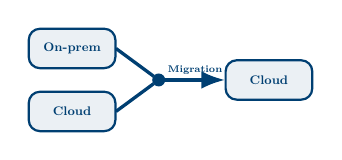
\begin{tikzpicture}[scale=0.5,every node/.style={transform shape}]
  \tikzstyle{env}=[draw=earlblue,thick,rounded corners,fill=earlblue!8,
    minimum width=2.2cm,minimum height=1cm,align=center,text=earlblue,font=\small\bfseries]
  % Source environments on the left
  \node[env] (onprem) at (0,0.8) {On-prem};
  \node[env] (cloudsrc) at (0,-0.8) {Cloud};
  % Central junction node
  \node[circle,draw=earlblue,fill=earlblue,minimum size=3mm,inner sep=0pt] (hub) at (2.2,0) {};
  % Destination cloud on the right
  \node[env] (dst) at (5,0) {Cloud};
  % Sources meet at the hub
  \draw[earlblue,very thick] (onprem.east) -- (hub);
  \draw[earlblue,very thick] (cloudsrc.east) -- (hub);
  % Hub points to the destination cloud
  \draw[-{Latex[length=3mm]},earlblue,very thick] (hub) -- (dst.west)
    node[midway,above,text=earlblue,font=\scriptsize\bfseries] {Migration};
\end{tikzpicture}
\end{center}
\end{column}
% -- Right: codebase to discovery report pipeline --
\begin{column}{0.58\textwidth}
\begin{center}
{\small\bfseries\color{earlblue}From codebase to discovery report}\\[0.15cm]
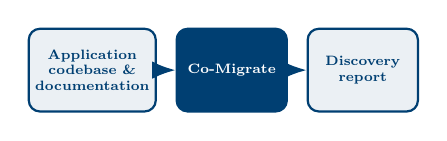
\begin{tikzpicture}[scale=0.7,every node/.style={transform shape},node distance=0.35cm]
  \tikzstyle{box}=[draw=earlblue,thick,rounded corners,fill=earlblue!8,
    minimum width=2cm,minimum height=1.5cm,align=center,text=earlblue,font=\scriptsize\bfseries]
  \tikzstyle{core}=[draw=earlblue,thick,rounded corners,fill=earlblue,
    minimum width=2cm,minimum height=1.5cm,align=center,text=white,font=\scriptsize\bfseries]
  \node[box] (input) {Application\\ codebase \&\\ documentation};
  \node[core,right=of input] (core) {Co-Migrate};
  \node[box,right=of core] (report) {Discovery\\ report};
  \draw[-{Latex[length=3mm]},earlblue,very thick] (input) -- (core);
  \draw[-{Latex[length=3mm]},earlblue,very thick] (core) -- (report);
\end{tikzpicture}
\end{center}
\end{column}
\end{columns}

\vspace{0.1cm}
{\small
\begin{itemize}
  \item \textbf{Discovery first:} every migration starts with a discovery stage to map dependencies and spot risks.
\end{itemize}
}

\vspace{0.05cm}
\begin{block}{\small The problems Co-Migrate solves}
{\footnotesize
\begin{itemize}
  \item \textbf{\color{earlblue}The bottleneck:} teams can spend \colorbox{earlblue!15}{up to \textbf{53 weeks}} on discovery alone - slow, manual and costly.
  \item \textbf{Risk matters early:} spotting risks and complexity up front is key to a successful migration.
\end{itemize}
}
\end{block}
\end{frame}

% =====================================================================
% 2. Data Preprocessing
% =====================================================================
\section{Data Preprocessing}
\begin{frame}
\frametitle{Data Preprocessing - Making Documentation AI-Ready}

\vspace{-0.15cm}
\begin{center}
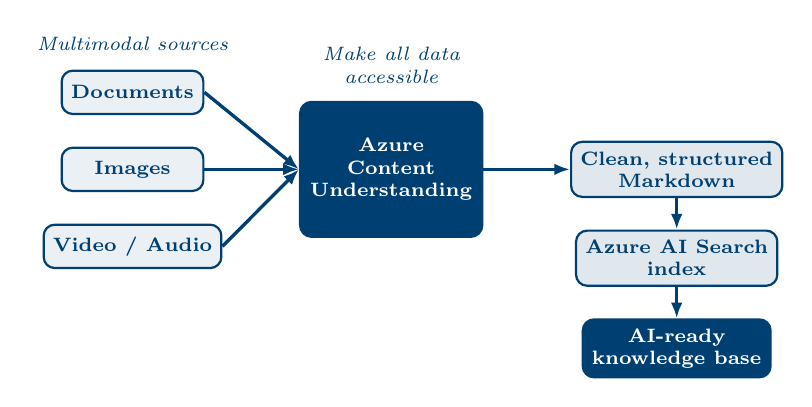
\begin{tikzpicture}[node distance=0.4cm,every node/.style={transform shape}]
  \tikzstyle{src}=[draw=earlblue,thick,rounded corners,fill=earlblue!8,
    minimum width=1.8cm,minimum height=0.55cm,align=center,text=earlblue,font=\scriptsize\bfseries]
  \tikzstyle{core}=[draw=earlblue,very thick,rounded corners,fill=earlblue,
    minimum width=2.3cm,minimum height=1.7cm,align=center,text=white,font=\scriptsize\bfseries]
  \tikzstyle{stage}=[draw=earlblue,thick,rounded corners,fill=earlblue!12,
    minimum width=2.3cm,minimum height=0.7cm,align=center,text=earlblue,font=\scriptsize\bfseries]
  \tikzstyle{flow}=[-{Latex[length=2mm]},earlblue,very thick]

  % -- Multimodal inputs (stacked) --
  \node[src] (docs)  {Documents};
  \node[src,below=of docs]   (imgs)  {Images};
  \node[src,below=of imgs]   (media) {Video / Audio};
  \node[above=0.12cm of docs,text=earlblue,font=\scriptsize\itshape] {Multimodal sources};

  % -- Azure Content Understanding (core) --
  \node[core,right=1.2cm of imgs] (cu) {Azure\\ Content\\ Understanding};
  \node[above=0.1cm of cu,text=earlblue,font=\scriptsize\itshape,align=center] {Make all data\\ accessible};

  % -- Right column: markdown -> search -> AI-ready (vertical chain) --
  \node[stage,right=1.1cm of cu] (md) {Clean, structured\\ Markdown};
  \node[stage,below=of md] (search) {Azure AI Search\\ index};
  \node[stage,below=of search,fill=earlblue,text=white] (ready) {AI-ready\\ knowledge base};

  % -- Flows --
  \draw[flow] (docs.east)  -- (cu.west);
  \draw[flow] (imgs.east)  -- (cu.west);
  \draw[flow] (media.east) -- (cu.west);
  \draw[flow] (cu.east) -- (md.west);
  \draw[flow] (md.south) -- (search.north);
  \draw[flow] (search.south) -- (ready.north);
\end{tikzpicture}
\end{center}

\vspace{-0.1cm}
{\footnotesize
\begin{itemize}
  \item \textbf{\color{earlblue}Content Understanding:} one analyzer for \emph{any} modality - OCR, layout, tables and figure descriptions turn messy files into clean Markdown.
  \item \textbf{\color{earlblue}Make all data accessible:} charts, diagrams and scans become searchable text, so nothing is lost to downstream agents.
  \item \textbf{\color{earlblue}Azure AI Search:} content is chunked and indexed into an AI-ready knowledge base for agentic retrieval.
\end{itemize}
}
\end{frame}

% =====================================================================
% 3. Inside Agentic Retrieval
% =====================================================================
\section{Inside Agentic Retrieval}
\begin{frame}
\frametitle{Inside Agentic Retrieval - A Multi-Query Pipeline}

\vspace{-0.15cm}
\begin{center}
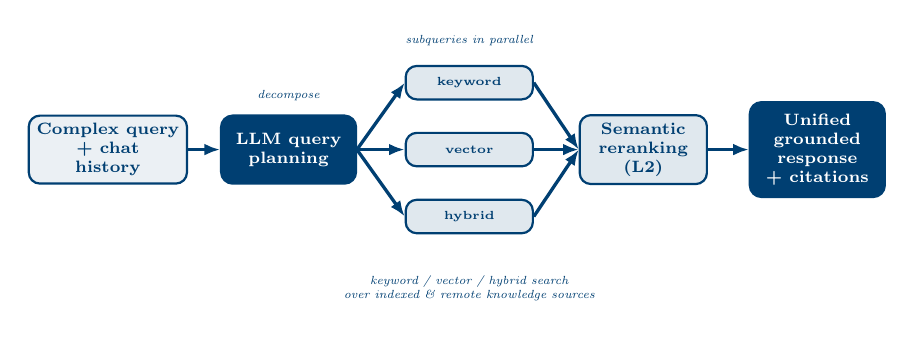
\begin{tikzpicture}[scale=0.85,every node/.style={transform shape}]
  \tikzstyle{io}=[draw=earlblue,thick,rounded corners,fill=earlblue!8,
    minimum width=2cm,minimum height=1cm,align=center,text=earlblue,font=\scriptsize\bfseries]
  \tikzstyle{core}=[draw=earlblue,very thick,rounded corners,fill=earlblue,
    minimum width=2cm,minimum height=1cm,align=center,text=white,font=\scriptsize\bfseries]
  \tikzstyle{sub}=[draw=earlblue,thick,rounded corners,fill=earlblue!12,
    minimum width=1.9cm,minimum height=0.5cm,align=center,text=earlblue,font=\tiny\bfseries]
  \tikzstyle{stage}=[draw=earlblue,thick,rounded corners,fill=earlblue!12,
    minimum width=1.9cm,minimum height=1cm,align=center,text=earlblue,font=\scriptsize\bfseries]
  \tikzstyle{flow}=[-{Latex[length=2mm]},earlblue,very thick]

  % -- Input --
  \node[io] (query) at (0,0) {Complex query\\ + chat\\ history};

  % -- LLM query planning --
  \node[core] (plan) at (2.7,0) {LLM query\\ planning};
  \node[above=0.08cm of plan,text=earlblue,font=\tiny\itshape,align=center] {decompose};

  % -- Parallel subqueries --
  \node[sub] (s1) at (5.4,1) {keyword};
  \node[sub] (s2) at (5.4,0) {vector};
  \node[sub] (s3) at (5.4,-1) {hybrid};
  \node[above=0.16cm of s1,text=earlblue,font=\tiny\itshape] {subqueries in parallel};

  % -- Semantic reranking --
  \node[stage] (rank) at (8,0) {Semantic\\ reranking\\ (L2)};

  % -- Merge / output --
  \node[core,minimum height=1.4cm] (resp) at (10.6,0) {Unified\\ grounded\\ response\\ + citations};

  % -- Flows --
  \draw[flow] (query.east) -- (plan.west);
  \draw[flow] (plan.east) -- (s1.west);
  \draw[flow] (plan.east) -- (s2.west);
  \draw[flow] (plan.east) -- (s3.west);
  \draw[flow] (s1.east) -- (rank.west);
  \draw[flow] (s2.east) -- (rank.west);
  \draw[flow] (s3.east) -- (rank.west);
  \draw[flow] (rank.east) -- (resp.west);

  % -- Knowledge sources note under subqueries --
  \node[below=0.5cm of s3,text=earlblue,font=\tiny\itshape,align=center]
    {keyword / vector / hybrid search\\ over indexed \& remote knowledge sources};
\end{tikzpicture}
\end{center}

\vspace{-0.05cm}
{\footnotesize
\begin{itemize}
  \item \textbf{\color{earlblue}Beyond classic RAG:} handles multi-part questions, chat context, typos and paraphrasing that a single query can't.
  \item \textbf{\color{earlblue}Query planning:} an LLM breaks the query down into focused subqueries that run \emph{in parallel}, each semantically reranked.
  \item \textbf{\color{earlblue}Grounded output:} best results are merged into one response with source citations and an activity log for agents.
\end{itemize}
}
\end{frame}

% =====================================================================
% 4. Agentic Orchestration
% =====================================================================
\section{Agentic Orchestration}
\begin{frame}
\frametitle{Agentic Orchestration - Overview}

\vspace{-0.1cm}
\begin{center}
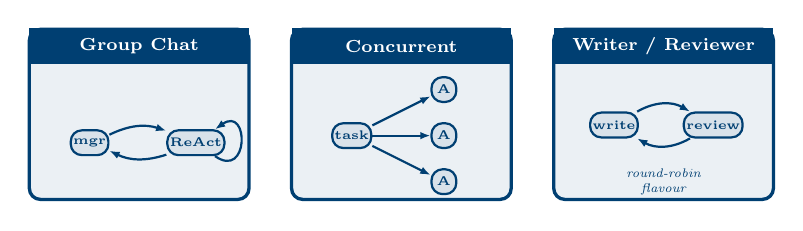
\begin{tikzpicture}[scale=0.9,every node/.style={transform shape}]
  \tikzstyle{card}=[draw=earlblue,very thick,rounded corners,fill=earlblue!8,
    minimum width=3.1cm,minimum height=2.4cm,align=center,text=earlblue]
  \tikzstyle{hd}=[fill=earlblue,text=white,font=\scriptsize\bfseries,
    minimum width=3.1cm,minimum height=0.5cm,align=center]
  \tikzstyle{mini}=[draw=earlblue,thick,rounded corners,fill=earlblue!15,
    minimum size=0.35cm,inner sep=1pt,text=earlblue,font=\tiny\bfseries]
  \tikzstyle{f}=[-{Latex[length=1.3mm]},earlblue,thick]

  % -- Card 1: Group Chat (1 manager + 1 ReAct agent) --
  \node[card] (c1) at (0,0) {};
  \node[hd,anchor=north] at (c1.north) {Group Chat};
  \node[mini] (m) at (-0.7,-0.4) {mgr};
  \node[mini] (a1) at (0.8,-0.4) {ReAct};
  \draw[f] (m) to[bend left=22] (a1);
  \draw[f] (a1) to[bend left=22] (m);
  \draw[f] (a1) to[out=-35,in=35,looseness=4] (a1);

  % -- Card 2: Concurrent --
  \node[card] (c2) at (3.7,0) {};
  \node[hd,anchor=north] at (c2.north) {Concurrent};
  \node[mini] (t) at (3.0,-0.3) {task};
  \node[mini] (b1) at (4.3,0.35) {A};
  \node[mini] (b2) at (4.3,-0.3) {A};
  \node[mini] (b3) at (4.3,-0.95) {A};
  \draw[f] (t) -- (b1); \draw[f] (t) -- (b2); \draw[f] (t) -- (b3);

  % -- Card 3: Writer / Reviewer --
  \node[card] (c3) at (7.4,0) {};
  \node[hd,anchor=north] at (c3.north) {Writer / Reviewer};
  \node[mini] (w) at (6.7,-0.15) {write};
  \node[mini] (r) at (8.1,-0.15) {review};
  \draw[f] (w) to[bend left=30] (r);
  \draw[f] (r) to[bend left=30] (w);
  \node[text=earlblue,font=\tiny\itshape,align=center] at (7.4,-0.95) {round-robin\\ flavour};
\end{tikzpicture}
\end{center}

\vspace{0.1cm}
{\footnotesize
\begin{itemize}
  \item \textbf{\color{earlblue}Framework:} Microsoft \textbf{Semantic Kernel} agent orchestration, tailored to our use case.
  \item \textbf{\color{earlblue}Two patterns:} \emph{Group Chat} (1 manager + 1 ReAct agent, custom termination) and \emph{Concurrent} (parallel, per-repo agents).
  \item \textbf{\color{earlblue}Writer/Reviewer} is a \emph{Round-Robin} flavour of Group Chat - same orchestration, alternating turns.
\end{itemize}
}
\end{frame}

\begin{frame}
\frametitle{Agentic Orchestration - Group Chat}

\vspace{-0.5cm}
\begin{center}
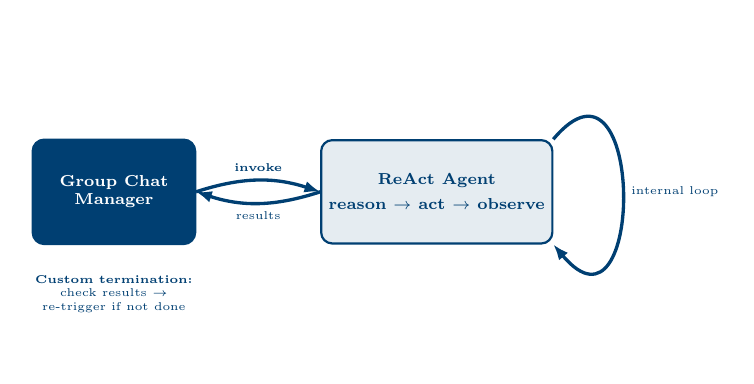
\begin{tikzpicture}[scale=0.82,every node/.style={transform shape}]
  \tikzstyle{core}=[draw=earlblue,very thick,rounded corners,fill=earlblue,
    minimum width=2.5cm,minimum height=1.6cm,align=center,text=white,font=\scriptsize\bfseries]
  \tikzstyle{ag}=[draw=earlblue,thick,rounded corners,fill=earlblue!10,
    minimum width=3cm,minimum height=1.6cm,align=center,text=earlblue,font=\scriptsize\bfseries]
  \tikzstyle{f}=[-{Latex[length=2mm]},earlblue,very thick]

  % -- Manager --
  \node[core] (mgr) at (0,0) {Group Chat\\ Manager};

  % -- Single ReAct agent --
  \node[ag] (agent) at (5,0) {\textbf{ReAct Agent}\\[3pt]\scriptsize reason $\to$ act $\to$ observe};
  % internal react loop
  \draw[f] (agent.north east) to[out=50,in=-50,looseness=3.5]
    node[right,font=\tiny,text=earlblue]{internal loop} (agent.south east);

  % -- invoke / results --
  \draw[f] (mgr.east) to[bend left=18] node[midway,above,font=\tiny\bfseries,text=earlblue]{invoke} (agent.west);
  \draw[f] (agent.west) to[bend left=18] node[midway,below,font=\tiny,text=earlblue]{results} (mgr.east);

  % -- custom termination --
  \node[below=0.35cm of mgr,align=center,font=\tiny,text=earlblue]
    {\textbf{Custom termination:}\\ check results $\to$\\ re-trigger if not done};
\end{tikzpicture}
\end{center}

\vspace{0.05cm}
{\footnotesize
\begin{itemize}
  \item \textbf{\color{earlblue}Our setup:} \emph{one} manager coordinating a \emph{single} ReAct agent - not a multi-agent debate.
  \item \textbf{\color{earlblue}Why a manager:} a ReAct agent's reason--act loop is trained to stop early; the manager inspects its results and \emph{re-triggers} the loop when the task isn't complete.
  \item \textbf{\color{earlblue}Net effect:} a custom termination strategy on top of the agent's own reason--act loop.
\end{itemize}
}
\end{frame}

\begin{frame}
\frametitle{Agentic Orchestration - Concurrent}

\vspace{-0.1cm}
\begin{center}
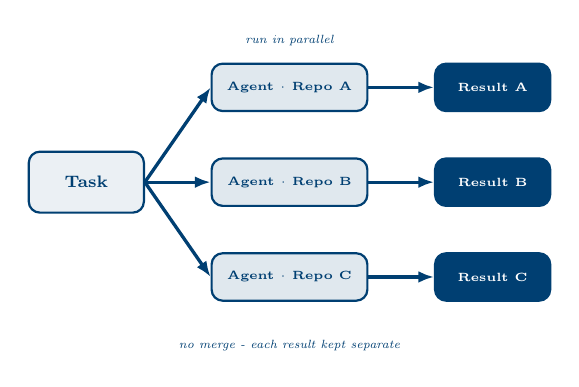
\begin{tikzpicture}[scale=0.86,every node/.style={transform shape}]
  \tikzstyle{io}=[draw=earlblue,thick,rounded corners,fill=earlblue!8,
    minimum width=1.7cm,minimum height=0.9cm,align=center,text=earlblue,font=\scriptsize\bfseries]
  \tikzstyle{ag}=[draw=earlblue,thick,rounded corners,fill=earlblue!12,
    minimum width=2.3cm,minimum height=0.7cm,align=center,text=earlblue,font=\tiny\bfseries]
  \tikzstyle{res}=[draw=earlblue,thick,rounded corners,fill=earlblue,
    minimum width=1.7cm,minimum height=0.7cm,align=center,text=white,font=\tiny\bfseries]
  \tikzstyle{f}=[-{Latex[length=2mm]},earlblue,very thick]

  \node[io] (task) at (0,0) {Task};

  \node[ag] (a1) at (3,1.4) {Agent $\cdot$ Repo A};
  \node[ag] (a2) at (3,0)   {Agent $\cdot$ Repo B};
  \node[ag] (a3) at (3,-1.4){Agent $\cdot$ Repo C};
  \node[above=0.12cm of a1,text=earlblue,font=\tiny\itshape] {run in parallel};

  \node[res] (o1) at (6,1.4) {Result A};
  \node[res] (o2) at (6,0)   {Result B};
  \node[res] (o3) at (6,-1.4){Result C};

  \draw[f] (task.east) -- (a1.west);
  \draw[f] (task.east) -- (a2.west);
  \draw[f] (task.east) -- (a3.west);
  \draw[f] (a1.east) -- (o1.west);
  \draw[f] (a2.east) -- (o2.west);
  \draw[f] (a3.east) -- (o3.west);

  \node[below=0.45cm of a3,text=earlblue,font=\tiny\itshape,align=center]
    {no merge - each result kept separate};
\end{tikzpicture}
\end{center}

\vspace{0.05cm}
{\footnotesize
\begin{itemize}
  \item \textbf{\color{earlblue}Our setup:} the task fans out to one agent \emph{per repo}, all running in parallel.
  \item \textbf{\color{earlblue}No aggregation:} results are \emph{not} combined - each agent only needs its own repo's context.
  \item \textbf{\color{earlblue}Benefits:} parallelism for speed, plus clean isolation - no cross-repo context bleed.
\end{itemize}
}
\end{frame}

\begin{frame}
\frametitle{Agentic Orchestration - Writer/Reviewer}

\vspace{-0.15cm}
\begin{columns}[T]
\begin{column}{0.5\textwidth}
\begin{center}
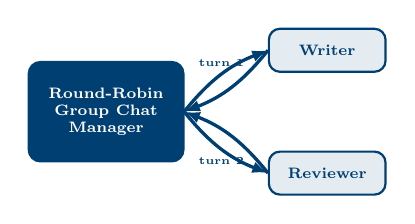
\begin{tikzpicture}[scale=0.78,every node/.style={transform shape}]
  \tikzstyle{core}=[draw=earlblue,very thick,rounded corners,fill=earlblue,
    minimum width=2.5cm,minimum height=1.6cm,align=center,text=white,font=\scriptsize\bfseries]
  \tikzstyle{ag}=[draw=earlblue,thick,rounded corners,fill=earlblue!10,
    minimum width=1.9cm,minimum height=0.7cm,align=center,text=earlblue,font=\scriptsize\bfseries]
  \tikzstyle{f}=[-{Latex[length=2mm]},earlblue,very thick]

  \node[core] (mgr) at (0,0) {Round-Robin\\ Group Chat\\ Manager};
  \node[ag] (w) at (3.6,1) {Writer};
  \node[ag] (r) at (3.6,-1) {Reviewer};

  \draw[f] (mgr.east) to[bend left=15] node[midway,above,font=\tiny\bfseries,text=earlblue]{turn 1} (w.west);
  \draw[f] (w.west) to[bend left=15] (mgr.east);
  \draw[f] (mgr.east) to[bend right=15] node[midway,below,font=\tiny\bfseries,text=earlblue]{turn 2} (r.west);
  \draw[f] (r.west) to[bend right=15] (mgr.east);
\end{tikzpicture}
\end{center}
\end{column}
\begin{column}{0.5\textwidth}
\begin{block}{\footnotesize What Round-Robin overrides}
{\scriptsize
\texttt{SelectNextAgent} - picks the next agent by a fixed \textbf{cyclic order} (a round-robin cursor).
\vspace{2pt}
\par{\color{earlblue}\itshape Everything else is inherited from the base \texttt{GroupChatManager}.}
}
\end{block}
\end{column}
\end{columns}

\vspace{0.55cm}
{\footnotesize
\begin{itemize}
  \item \textbf{\color{earlblue}Same pattern:} reuses the \emph{Group Chat} orchestration with the \texttt{RoundRobinGroupChatManager} flavour - no custom manager logic needed.
  \item \textbf{\color{earlblue}Deterministic turns:} Writer drafts, Reviewer critiques, alternating for a fixed number of rounds (writer gets the last word).
  \item \textbf{\color{earlblue}Benefits:} a built-in quality gate - iterative critique lifts output quality with predictable turns and no custom manager logic.
\end{itemize}
}
\end{frame}

% =====================================================================
% 5. Agents' Memory
% =====================================================================
\section{Agents' Memory}
\begin{frame}
\frametitle{Agents' Memory}
\begin{itemize}
  \item \textbf{What it is:} \emph{placeholder} -
  \item \textbf{How it works:} \emph{placeholder} - co-located \texttt{.agent.md} prompt, agent-owned memory, shared memory.
  \item \textbf{Where used:} \emph{placeholder} - discovery
\end{itemize}
\end{frame}  

% =====================================================================
% 6. Agents' Tools
% =====================================================================
\section{Agents' Tools}
\begin{frame}
\frametitle{Agents' Tools}
\begin{itemize}
  \item \textbf{Agent anatomy:} factory \texttt{get\_X\_agent()}, co-located \texttt{.agent.md} prompt, agent-owned tools.
  \item \textbf{Tool catalogue:} \texttt{discovery\_memory}, \texttt{file\_system}, \texttt{search}, \texttt{grounding}, \texttt{ado\_docs}, \texttt{sdp\_docs}.
  \item \textbf{Shared middleware:} \emph{placeholder} - Agent / Function / Chat / TokenUsage logging.
\end{itemize}
\end{frame}

% =====================================================================
% 7. Agent-as-a-tool Pattern
% =====================================================================
\section{Agent-as-a-tool Pattern}
\begin{frame}
\frametitle{Agent-as-a-tool Pattern}
\begin{itemize}
  \item \textbf{Concept:} \emph{placeholder} - exposing an agent as a callable tool for another agent.
  \item \textbf{Why:} \emph{placeholder} - composition, encapsulation, reuse.
  \item \textbf{Example:} \emph{placeholder}.
\end{itemize}
\end{frame}

% =====================================================================
% 8. E2E Orchestration Phases
% =====================================================================
\section{E2E Orchestration Phases}
\begin{frame}
\frametitle{E2E Orchestration Phases - Overview}
\begin{center}
Discovery $\to$ Deep Analysis $\to$ Enterprise Context $\to$ UAQ $\to$ Reporting $\to$ Cleanup
\end{center}
\emph{placeholder} - how the phases hand off state end-to-end.
\end{frame}

\begin{frame}
\frametitle{Discovery Phase}
\begin{itemize}
  \item \textbf{Goal:} \emph{placeholder}.
  \item \textbf{Agents \& tools:} \emph{placeholder}.
  \item \textbf{Output:} \emph{placeholder} - discovery memory.
\end{itemize}
\end{frame}

\begin{frame}
\frametitle{Deep Analysis Phase}
\begin{itemize}
  \item \textbf{Goal:} \emph{placeholder}.
  \item \textbf{Orchestration:} concurrent batches.
  \item \textbf{Output:} \emph{placeholder}.
\end{itemize}
\end{frame}

\begin{frame}
\frametitle{Enterprise Context Phase}
\begin{itemize}
  \item \textbf{Goal:} \emph{placeholder} - enrich with LSEG/enterprise context.
  \item \textbf{Sources:} \emph{placeholder}.
  \item \textbf{Output:} \emph{placeholder}.
\end{itemize}
\end{frame}

\begin{frame}
\frametitle{Unified Assessment Questionnaire (UAQ) Phase}
\begin{itemize}
  \item \textbf{Goal:} \emph{placeholder} - Unified Assessment Questionnaire.
  \item \textbf{Orchestration:} category-scoped concurrent agents.
  \item \textbf{Output:} \emph{placeholder}.
\end{itemize}
\end{frame}

\begin{frame}
\frametitle{Reporting Phase}
\begin{itemize}
  \item \textbf{Goal:} \emph{placeholder} - final recommendation report.
  \item \textbf{Orchestration:} writer/reviewer loop.
  \item \textbf{Output:} \emph{placeholder}.
\end{itemize}
\end{frame}

% =====================================================================
% 9. Application overview
% =====================================================================
\section{Application overview}
\begin{frame}
\frametitle{Application overview}
\begin{itemize}
  \item \textbf{High-level architecture:} \emph{placeholder} - diagram.
  \item \textbf{Stack:} Python 3.12, FastAPI, Poetry; React 19 frontend.
  \item \textbf{Data flow:} ingestion $\to$ preprocessing $\to$ agentic retrieval $\to$ orchestration.
\end{itemize}
\end{frame}

% =====================================================================
% 10. Infrastructure
% =====================================================================
\section{Infrastructure}
\begin{frame}
\frametitle{Infrastructure}
\begin{itemize}
  \item \textbf{Azure services:} \emph{placeholder} - Blob / Table / Queue, AI Search, Key Vault, Foundry OpenAI.
  \item \textbf{Deployment:} \emph{placeholder}.
  \item \textbf{Air-gapped considerations:} offline Mermaid CLI rendering, no remote fallback.
\end{itemize}
\end{frame}

% =====================================================================
% 11. Backend
% =====================================================================
\section{Backend}
\begin{frame}
\frametitle{Backend}
\begin{itemize}
  \item \textbf{API:} \emph{placeholder} - FastAPI endpoints.
  \item \textbf{Reliability:} \texttt{retry.py} ErrorClass (transient / deterministic / partial), exponential backoff + jitter.
  \item \textbf{Observability:} \emph{placeholder} - OpenTelemetry token metrics.
\end{itemize}
\end{frame}

% =====================================================================
% 12. Frontend
% =====================================================================
\section{Frontend}
\begin{frame}
\frametitle{Frontend}
\begin{itemize}
  \item \textbf{Stack:} React 19.
  \item \textbf{Key views:} \emph{placeholder}.
  \item \textbf{UX flow:} \emph{placeholder}.
\end{itemize}
\end{frame}

% -- Closing --
\begin{frame}
\frametitle{Questions}
\begin{center}
\Large Thank you - Questions?
\end{center}
\end{frame}

\end{document}